\chapter{Planificaci�n del trabajo} 
\label{chap:schedule}
\section{Diagrama de actividades}
En mi opini�n este proyecto no cuadra con el esquema de un ciclo de vida convencional, esto se debe a que nuestro trabajo consiste en la extensi�n de una herramienta ya existente, como es ArgoSPE. Se ha considerado m�s adecuado describir el modo en que se ha desarrollado mi trabajo gracias a un esquema que tiene mucha similitud con un ciclo de vida en cascada mejorado. La siguiente figura representa el orden cronol�gico de las fases (ver \ref{sec:fases} y \ref{sec:trabajo}) en las se organiz� mi proyecto desde el primer momento.

\begin{figure}[H]
	\begin{center}
		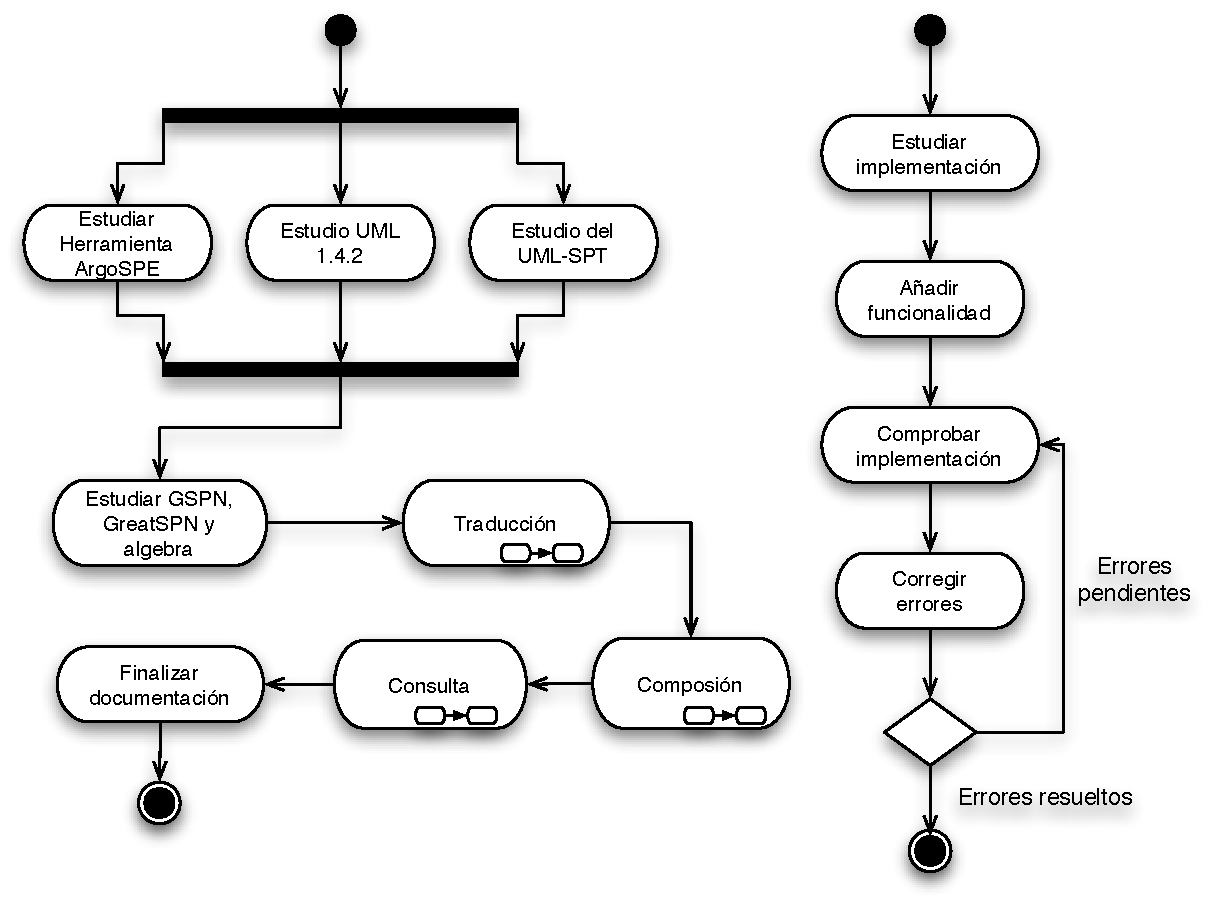
\includegraphics[scale=0.7]{planificacion.pdf}
	\end{center}
	\caption{Diagramas de actividades de la planificaci�n.}
	\label{fig:planificacion}
\end{figure}

\section{Diagrama de Gantt}

\begin{figure}[H]
	\begin{center}
		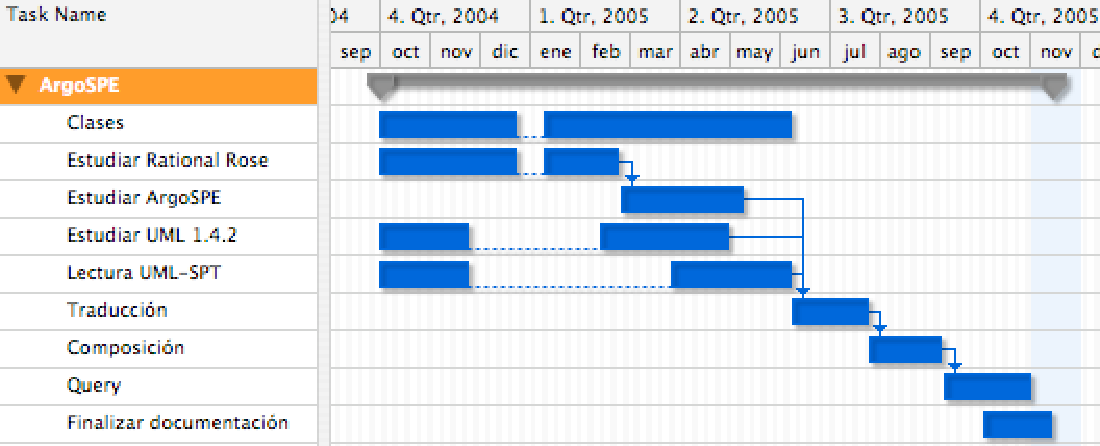
\includegraphics[scale=0.75]{shortgantt.pdf}
	\end{center}
	\caption{Diagrama de la cronolog�a real.}
	\label{fig:gantt}
\end{figure}

En el diagrama anterior queda reflejado (tarea Clases) el hecho de que durante la realizaci�n de este proyecto he tenido que terminar las �ltimas asignaturas de mi carrera,  factor que ha supuesto la prolongaci�n, m�s all� de lo esperado, de algunas tareas relacionadas con mi trabajo.

Otro hecho muy importante que ha marcado el transcurso de mi trabajo fue {\bf estudio de Rational Rose}\footnote{El objetivo original del proyecto era modificar ArgoSPE para que trabajara con Rational Rose.} \cite{Rose}, que consisiti� en la b�squeda y lectura de toda la informaci�n disponible referente a la extensi�n de esta aplicaci�n.

La investigaci�n realizada concluy� con, la implementaci�n de una peque�a extensi�n, en forma de submen�, y con la idea clara de que era {\bf imposible}\footnote{Este t�rmino refleja el hecho de que no disponer de la documentaci�n adecuada prolongar�a en exceso una posible extensi�n, haciendo inviable esa opci�n.} llegar a desarrollar una extensi�n completa, a menos que fu�ramos socios tecnol�gicos de la empresa\footnote{Rational, la empresa desarrolladora, fue adquirida por IBM.} que se dedicaba a la implementaci�n de la herramienta, puesto que la documentaci�n necesaria para ello solamente era distribu�da a estos �ltimos.

El resultado de la investigaci�n hizo que el objetivo de mi proyecto fuera completamente diferente al que en un principio se me hab�a propuesto, a partir de ahora nuestro trabajo iba a consistir en la ampliaci�n de la herramienta ArgoSPE.

A parte de hacer inservible la gran parte del trabajo elaborado en la primera fase, estos cambios produjeron una reestructuraci�n completa de las tareas que se deb�an realizar para conseguir los nuevos objetivos, estas nuevas tareas son las que aparecen en el diagrama anterior a partir de Febrero de 2005.

El gr�fico anterior pone de manifiesto las dependencias existentes entre las tareas en las cuales se ha organizado el trabajo, as� se puede observar que el estudio de la teor�a precede a la implementaci�n de cada una de las partes. Tambi�n observamos que, existe una dependencia entre la traducci�n, la composici�n y la consulta, la cual ha sido respetada.